\scanpage{70}
% archive sheet number: 69
% Several long oblique cancellation strokes cross the draft.
\deleted{\uline{Exemples} 7.5.3. \mbox{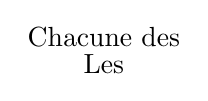
\begin{tikzpicture}[baseline=(base.base)]
\node[inner sep=0] (base) {\deleted{Les}};
\node[anchor=south,inner sep=0,yshift=.08cm,xshift=0cm] at (base.north) {\inserted{Chacune des}};
\end{tikzpicture}} propriétés \raisebox{1.7ex}{\inserted{\uuline{R}}} suivantes satisfait aux \mbox{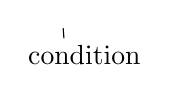
\begin{tikzpicture}[baseline=(word.base)]
\node[inner sep=0] (word) {condition};
\path (word.north west) -- coordinate[pos=.32] (mark) (word.north east);
% Isolated short brownish vertical trace; no letter or function assigned.
\draw[line width=.4pt] ([yshift=.08cm]mark) -- ([yshift=.21cm,xshift=-.01cm]mark);
\end{tikzpicture}} a) et b) de 7.5.1., \deleted{pourvu que $B$ soit un} lorsque $B$ est un excellent anneau:}
\begin{enumerate}
\item[\deleted{(i)}] \deleted{$\operatorname{coprof}C\quad n$}
\item[\deleted{(ii)}] \deleted{$S_n$}
\item[\deleted{(iii)}] \deleted{Coh Mac}
\item[\deleted{(iv)}] \deleted{régulier}
\item[\deleted{(v)}] \deleted{normal $R_n$}
\item[\deleted{(vi)}] \deleted{normal}
\item[\deleted{(vii)}] \deleted{intègre}
\item[\deleted{(viii)}] \deleted{réduit}
\end{enumerate}

\deleted{En fait, pour (vii) et (viii) c'est vrai sans aucune hypothèse sur $B$, pour (i) (ii) (iii) il suffit de \mbox{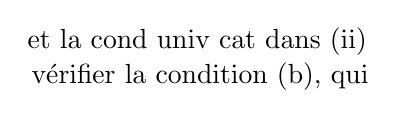
\begin{tikzpicture}[baseline=(base.base)]
\node[inner sep=0] (base) {vérifier la condition (b), \deleted{qui}};
\node[anchor=south west,inner sep=0,yshift=.08cm,xshift=-.05cm] at (base.north west) {\inserted{et la cond univ cat dans (ii)}};
\end{tikzpicture}} ce \mbox{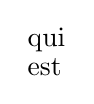
\begin{tikzpicture}[baseline=(base.base)]
\node[inner sep=0] (base) {est};
\node[anchor=south west,inner sep=0,yshift=.08cm,xshift=0cm] at (base.north west) {\inserted{qui}};
\end{tikzpicture}} vérifiéé si \deleted{\unsure{tout|tant} que} $B$ est quotient d'un régulier, ou satisfait la condition de Nagata sur le \mbox{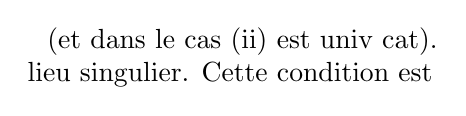
\begin{tikzpicture}[baseline=(base.base)]
\node[inner sep=0] (base) {lieu singulier. Cette condition est};
\node[anchor=south west,inner sep=0,yshift=.08cm,xshift=.25cm] at (base.north west) {\inserted{(et dans le cas (ii) est univ cat).}};
\end{tikzpicture}} également suffisante pour faire marcher (iv) (v) (vi), pourvu que dans (v) et (vi) on suppose de plus $B$ universellement caté\rlap{h}naire. Enfin, pour faire marcher (vi), on peut aussi prendre la condition ``$B$ est univ japonais et univ cat''.}
\margin{\deleted{\mbox{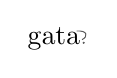
\begin{tikzpicture}[baseline=(word.base)]
\node[inner sep=0] (word) {gata};
% Faint extra curved impression and lower spot at the right of the last a; identity/function uncertain.
\draw[line width=.35pt,opacity=.65] ([xshift=-.05cm,yshift=.10cm]word.east) .. controls ([xshift=.09cm,yshift=.11cm]word.east) and ([xshift=.10cm,yshift=.03cm]word.east) .. ([xshift=.02cm,yshift=-.01cm]word.east);
\fill[opacity=.65] ([xshift=.04cm,yshift=-.05cm]word.east) circle (.015cm);
\end{tikzpicture}}}}

\deleted{\uline{Remarques} 7.5.4.\quad (i) comme 7.5.6. (i)}

\deleted{(ii) Comme 7.5.6. (ii) ; il s'agirait pratiquement des propriétés (i) \deleted{(ii)} (iii) (vii) ou (viii).}

\deleted{(iii) Dans la situation 7.5.1., on dispose le plus souvent d'une propriété supplémentaire de \uuline{R}, garantissant que si \deleted{$A\quad B$} $\text{\uuline{R}}(A)$ est vrai et les fibres de $\operatorname{Spec}(B)\quad\operatorname{Spec}(A)$ satisfont la condition \uuline{R} géométrique, \deleted{il en est de même} alors \deleted{($\operatorname{Spec}(B)$ étant} ($B$ étant plat sur $A$, rappelons-le) $\text{\uuline{R}}(B)$ est vrai. On peut donc ti\rlap{e}rer de 7.5.1. que}
